%%%%%%%%%%%%%%%%%%%%%%%%%%%%%%%%%%%%%%%%%%%%%%%%%%%%%%%%%%%%%%%%%%%%%%%%%%%%%%%%
%% Packages
%%%%%%%%%%%%%%%%%%%%%%%%%%%%%%%%%%%%%%%%%%%%%%%%%%%%%%%%%%%%%%%%%%%%%%%%%%%%%%%%

%% Define class. Article is a simple one useful for most documents.
\documentclass{article}

%% Page formatting
\pagestyle{plain}
\usepackage{fullpage}                       %1in margins
\usepackage{titling}                        %Left align title
\pretitle{\begin{flushleft}\Large}
\posttitle{\par\end{flushleft}}
\preauthor{\begin{flushleft}\large}
\postauthor{\end{flushleft}}
\predate{\begin{flushleft}\large}
\postdate{\end{flushleft}}

%% Citations
\usepackage{hyperref} %Add link to actual website
\usepackage{url}      %Text display of urls

%% Mathematics
\usepackage{amsthm, amssymb, amsmath}

\usepackage{graphicx}
\graphicspath{ {images/} }




%% Title information
\title{CMSC 221 - Fall 2017 - Project 3: Results and Analysis} %Specify homework number
\author{Palmer Robins}                         %Put your name
\date{November 29, 2017}                       %Put due date

\begin{document}

% First things first, make your title!
\maketitle

% Use an enumeration for your answers. One \item per problem in order as
% specified online.

\section{Introduction.}

    \vskip 1em
    In this experiment we compared several different sorting algorithms. We implemented bubble sort, 
    at least one slow sort, as well as at least one fast sort. Through timing these algorithms, we would
    be able to visualize the importance of, in the case of large data sets, using a faster sorting 
    algorithm in order to gain greater efficiency. I learned the importance of knowing what you need
    sorted is important in choose an option; if you only have to sort a handful of elements, a slow sort
    will work just fine. However, if thousands of elements are involved, a quick sort is most definitely 
    needed. 
    \vskip 1em

\section{Implementation Details.}

   \vskip 1em
   I implemented bubble sort, selection sort (slow sort), and heap sort (fast sort). We had the helper 
   function $swap()$ and a comparator to aid in each implementation. In the heap sort
   implementation, I created a second function, $heapify()$, which is a fundamental aspect of heap 
   sort which is called by the heap sort function. I also implemented insertion sort after completing 
   the main requirements of the assignment. 
   \vskip 1em

\section{Theoretical Analysis.}
  \vskip .5em
  
  Luckily, these sorting algorithms below run at the same theoretical complexity no matter the 
  case. However, in the analysis below it's clear that one should be running much quicker than 
  the other two. Bubble sort is one of the slowest possible sorting algorithms out there, which is 
  evident in its time complexity, just like Selection sort. However, heap sort sorts by inserting 
  into a heap, and runs in $O(nlog(n))$ time. 
    
   \vskip 1em
   {\bf Bubble Sort:} 
   \vskip .5em
   {\bf Best Case/Average Case/Worst Case -} In this implementation, all of these will by $O(n^2)$ for
   the bubble sort function. It's possible to implement a version that has linear time complexity 
   for an ordered list, but our implementation always runs in $O(n^2)$ time,  
   where $n$ is the number of elements to be sorted. Bubble sort will go through the entire list, 
   and at each item, it will go through the entire list again in order to "bubble" the item to
   the correct location.
   \vskip 1em
   
   {\bf Selection Sort:}
   \vskip .5em
   {\bf Best Case/Worst Case/Average Case -} Selection sort will always be $O(n^2)$ in every case.
   It scans through the $n$ elements to find the lowest value, then swaps that to the front. Then, it
   scans the remaining $n - 1$ unsorted elements to get the next lowest, until it's finished sorting.
   This simplifies to $O(n^2)$.
   \vskip 1em
   \newpage
   
   {\bf Heap Sort:}
   \vskip .5em
   {\bf Worst Case/Best Case/Average Case -} Heap sort runs in $O(n log(n))$ time. It takes logarithmic time to insert each element of the $n$
   needed to be sorted, and we're inserting $n$ times. We're able to insert much faster than the 
   quadratic algorithms due to the properties of a heap structure; it's much easier to find the 
   correct position within the heap. 
   \vskip 1em
  
\section{Experimental Setup}
    
    \vskip 1em
    The goal for this experiment was to time each sorting algorithm with four different cases. One 
    with a random order, one with elements already sorted, one with the elements in descending 
    order, and one with just a few unique elements. Through this test, we will be able to see 
    strengths and weaknesses of the three algorithms we're testing. Then, we can compare our 
    test results to the theoretical analysis above to check for correctness. \\
    \\
    Since actual time is dependent on hardware, here are the machine specifications: MacOS High
    Sierra 10.13, 16GB 19677 DDR3 RAM, Intel 2.9 GHz Core i5 
    processor. 
    
\section{Results and Discussion.} 
    \vskip 1em
   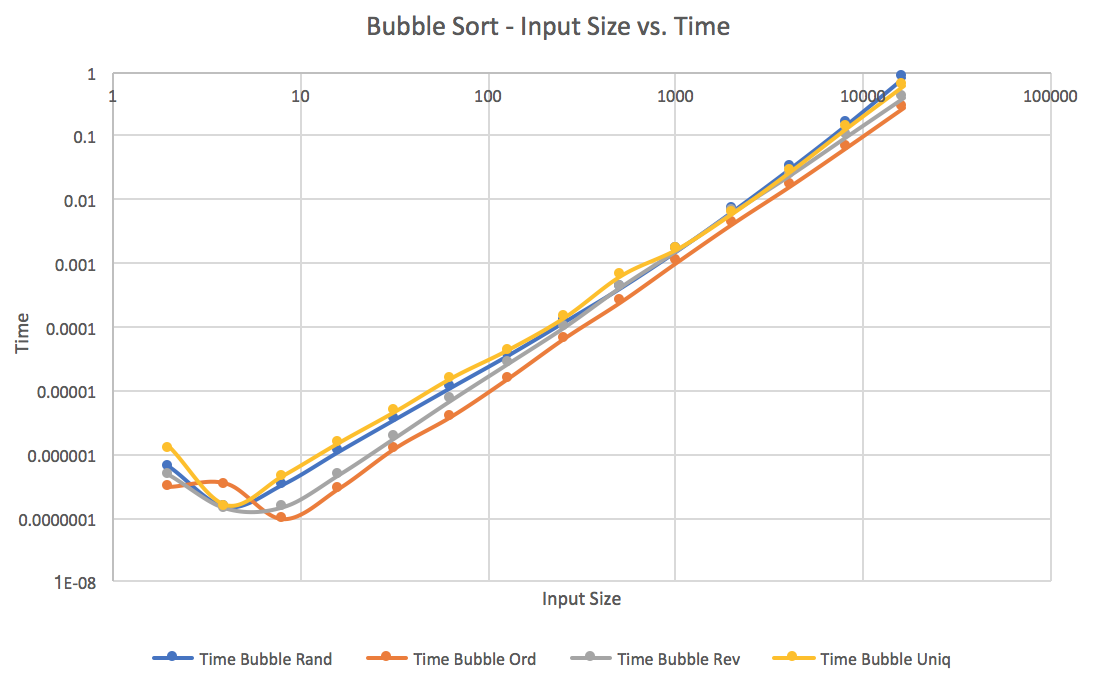
\includegraphics[scale = .70]{bs1}
   \vskip 1em
   \begin{tabular}{ | c || c | c | } 
   \hline
   Bubble Sort Input Type & $n_0$ & $c$ \\
   \hline\hline
   Random & 8 & 1.17E-05 \\
   \hline
   Ordered & 8 & 6.63E-05 \\
   \hline
   Reversed & 8 & 7.32E-06 \\
   \hline
   Unique Elements & 8 & 6.40E-04\\
   \hline
   \end{tabular}
    \vskip 1em
    This slow implementation of bubble has the same time complexity in every case, which results in
    similar linear trends from each type of input tested. Our theoretical time complexity is $O(n^2)$, 
    which is compared to the actual time in the graph below. 
    \vskip 1em
    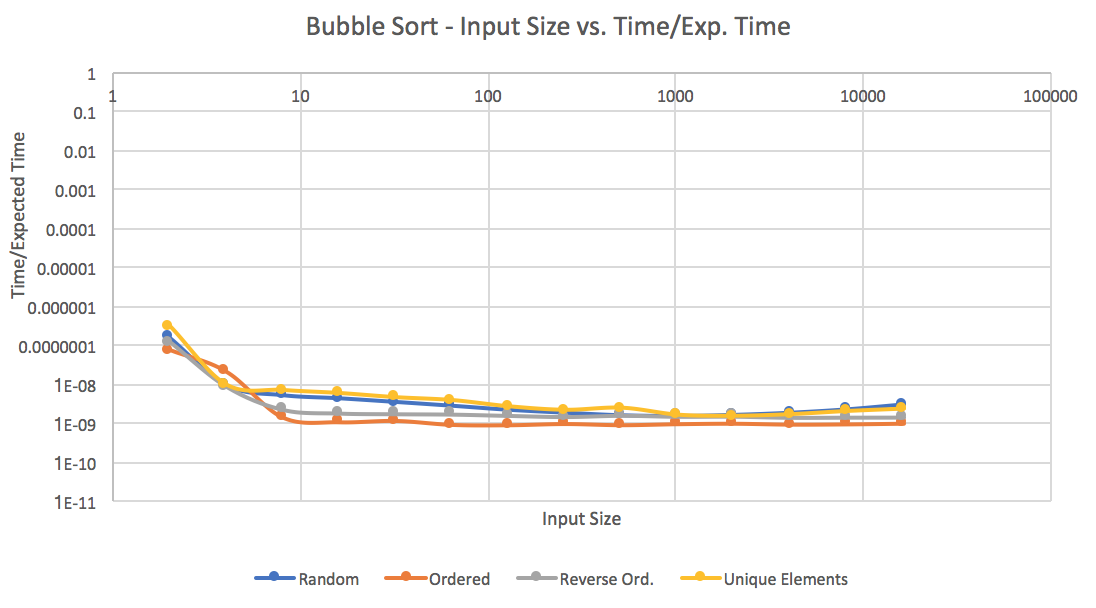
\includegraphics[scale = .70]{bs2}
    \vskip 1em
   \begin{tabular}{ | c || c | c | } 
   \hline
   Bubble Sort Input Type & $n_0$ & $c$ \\
   \hline\hline
   Random & 8 & 5.35148E-09 \\
   \hline
   Ordered & 8 & 1.01E-09 \\
   \hline
   Reversed & 8 & 1.82702E-09 \\
   \hline
   Unique Elements & 8 & 2.44033E-09\\
   \hline
   \end{tabular}
    \vskip 1em
    This graph proves the accuracy for our theoretical analysis for bubble sort. We put every actual time
    measurement over the theoretical time, which resulted in a nearly horizontal graph for each test, 
    meaning that the actual time is indeed very close to $O(n^2)$.
    \vskip 1em
    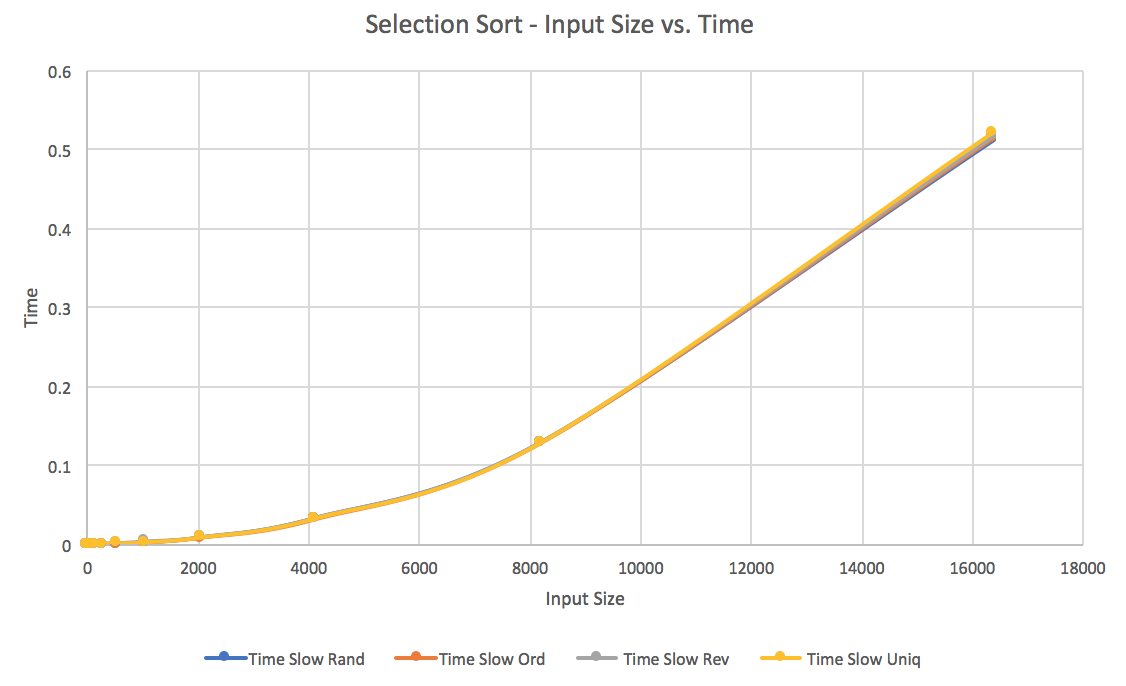
\includegraphics[scale = .70]{ss1}
    \vskip 1em
   \begin{tabular}{ | c || c | c | } 
   \hline
   Selection Sort Input Type & $n_0$ & $c$ \\
   \hline\hline
   Random & 2048 & 0.128142486 \\
   \hline
   Ordered & 2048 & 0.128142486 \\
   \hline
   Reversed & 2048 & 0.128142486 \\
   \hline
   Unique Elements & 2048 & 0.128142486\\
   \hline
   \end{tabular}
    \vskip 1em
    This graph also tested the same 4 types of inputted data, and not surprising resulted in nearly the 
    exact same results for each type. This is a good sign because selection sort, like bubble sort, will not
    have differing best, worst, and average cases. 
    \vskip1em
    
    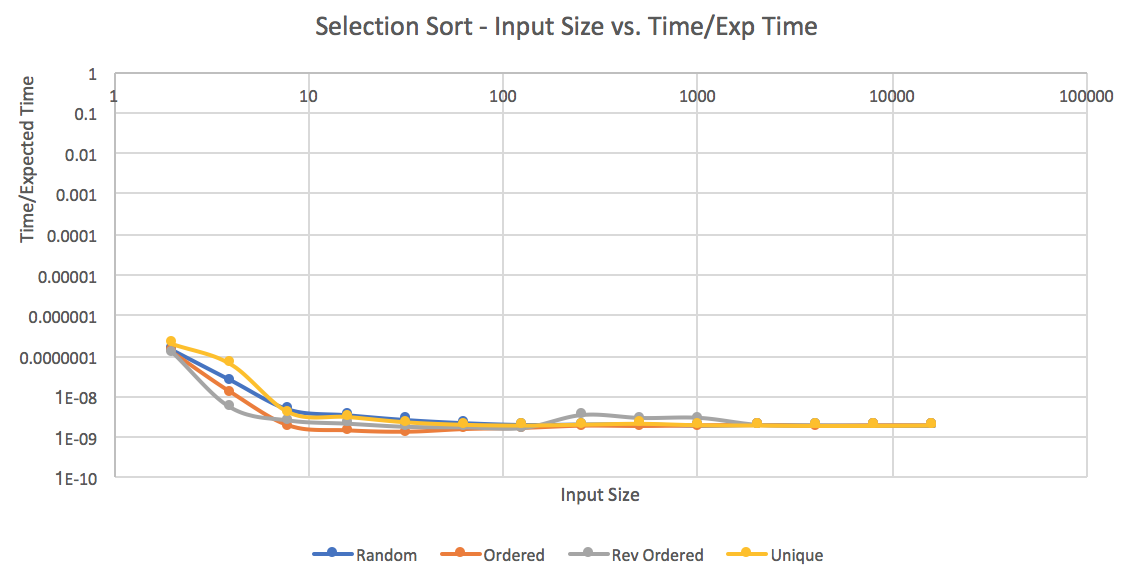
\includegraphics[scale = .70]{ss2}
    \vskip 1em
    \begin{tabular}{ | c || c | c | } 
   \hline
   Selection Sort Input Type & $n_0$ & $c$ \\
   \hline\hline
   Random & 8 & 2.02385E-09 \\
   \hline
   Ordered & 8 & 2.02385E-09 \\
   \hline
   Reversed & 8 & 3.48305E-09 \\
   \hline
   Unique Elements & 8 & 0.128142486\\
   \hline
   \end{tabular}
    \vskip 1em
    Each case is running in $O(n^2)$ time, according this graph where we set actual time to be divided
    by theoretical time. So, it isn't really much of an improvement over bubble sort; its still extremely 
    slow relative to the faster options available. 
    \vskip 1em
    
    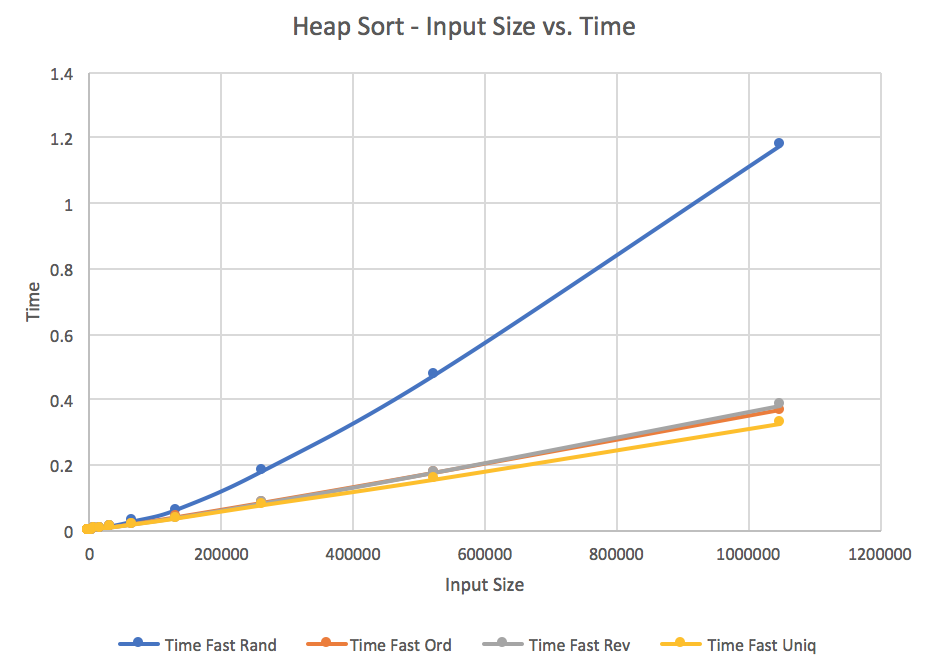
\includegraphics[scale = .70]{hs1}
    \vskip 1em
    \begin{tabular}{ | c || c | c | } 
   \hline
   Heap Sort Input Type & $n_0$ & $c$ \\
   \hline\hline
   Random & 256 & 0.180410165 \\
   \hline
   Ordered & 256 & 0.081187852 \\
   \hline
   Reversed & 256 & 0.081187852\\
   \hline
   Unique Elements & 256 & 0.076328125\\
   \hline
   \end{tabular}
    \vskip 1em
    In heap sort, we actually have to think about the different types of data and how they could effect
    time complexity. In our implementation, adding in a random order resulted in a less efficient trend 
    than the other three cases. Therefore, the blue line in this graph is the worst case for heap sort. 
    The other cases are all the best/averages cases (reversed, in-order, unique elements). 
    \vskip 1em
    
    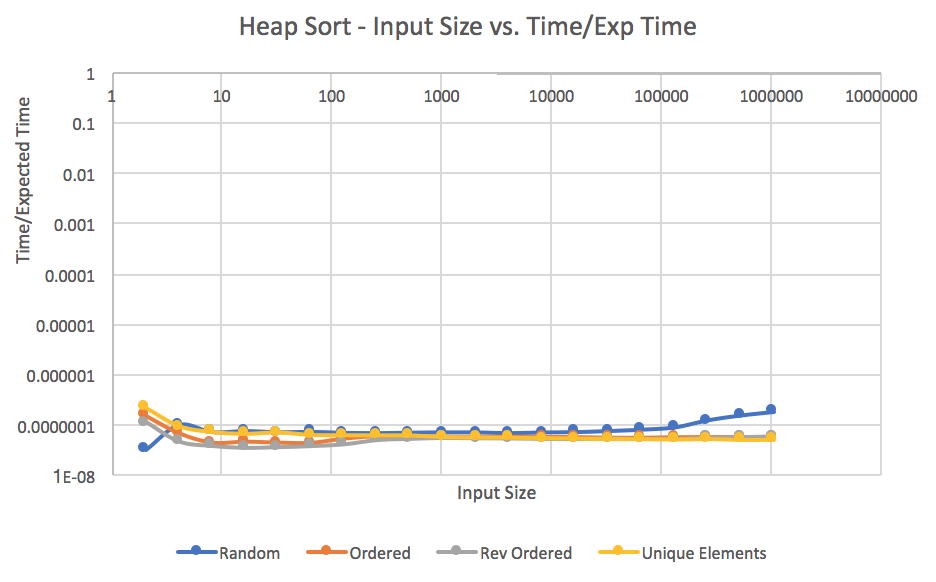
\includegraphics[scale = .70]{hs2}
    \vskip 1em
    \begin{tabular}{ | c || c | c | } 
   \hline
   Heap Sort Input Type & $n_0$ & $c$ \\
   \hline\hline
   Random & 8 & 7.31631E-08 \\
   \hline
   Ordered & 8 & 5.95051E-08 \\
   \hline
   Reversed & 8 & 5.66578E-08\\
   \hline
   Unique Elements & 8 & 5.91822E-08\\
   \hline
   \end{tabular}
    \vskip 1em
    The three better cases for heap sort are running in $O(nlog(n))$ time, whereas the worst case, 
    adding randomly ordered elements, is running in $O(n^2)$ time. Since each line is horizontal, 
    this analysis is proven correct.
    \vskip 1em
    
\section{Conclusion.}
	\vskip 1em
	A critical aspect of choosing a sorting algorithm is being aware of the properties of the data 
	you to sort. For example, if your data sets are mostly in order with just a few outliers, you could
	probably get away with simply using bubble sort, where the outliers will be fixed (assuming its 
	implemented to run in $O(n)$ for sorted data, unlike this implementation). If the data set is huge 
	and extremely out of order, you'll certainly need a fast sort of some kind. Understanding your data
	in question as well as the time complexities of all the options can help determine the exact sorting
	algorithm to use in a real world scenario. 

\end{document}
